\begin{definition}[Calculus Definition for Continuity] \leavevmode \\
    Let $(X,d)$ and $(Y, \overset{\sim}{d})$ be metric spaces. Let $E \subseteq X, ~c \in E',$ and $f: E \to Y$. We say $f$ is continuous at $c$ if all the following three conditions hold:
    \begin{enumerate}[$(i)$]
        \item $c \in E ~(\text{$f$ is defined at $c$})$
        \item $\lim \limits_{x \to c}f(x)$ exists
        \item $\lim \limits_{x \to c}f(x) = f(c)$
    \end{enumerate}
\end{definition}

\begin{remark}
    Let $f: E\subseteq (X, d) \to (Y, \overset{\sim}{d})$, and let $c \in E \cap E'.$ Then the following statements are equivalent:
    \begin{enumerate}[$(i)$]
        \item $\lim \limits_{x\to c}f(x) = f(c)$
        \item $\forall \epsilon > 0 ~\exists \delta > 0 \st \text{if $d(x,c) < \delta ~(x \in E),$ then $\overset{\sim}{d}(f(x), f(c)) < \epsilon$}$
        \item $\forall \epsilon > 0 ~\exists \delta > 0 \st \text{if $\forall x \in \nbhds{\delta}{X}{c}\cap E,$ then $f(x) \in \nbhds{\epsilon}{Y}{f(c)}$}$
        \item For every $\epsilon$-neighborhood $\nbhds{\epsilon}{Y}{f(c)}$ of $f(c)$, there exists a $\delta$-neighborhood $\nbhds{\delta}{X}{c}$ of $c \st$the image of $\nbhds{\delta}{X}{c}\cap E$ is contained in $\nbhds{\epsilon}{Y}{f(c)}.$
    \end{enumerate}
\end{remark}

\begin{definition}[General Definition of Continuity] \leavevmode \\
    Let $(x,d)$ and $(Y, \overset{\sim}{d})$ be two metric spaces, and let $E$ be a nonempty set in $X$. Let $c \in E$ and $f: E \to Y$. We say $f$ is continuous at $c$ if any of the following equivalent statements hold:
    \begin{enumerate}[$(i)$]
        \item $\forall \epsilon > 0 ~\exists \delta > 0 \st \text{ if $d(x,c) < \delta,$ then $\overset{\sim}{d}(f(x), f(c)) < \epsilon$}$
        \item $\forall \epsilon > 0 ~\exists \delta > 0 \st \forall x \in \nbhds{\delta}{X}{c}\cap E ~~f(x)\in \nbhds{\epsilon}{Y}{f(c)}$
        \item For every $\epsilon$-neighborhood $\nbhds{\epsilon}{Y}{f(c)}$ of $f(c)$, there exists a $\delta$-neighborhood $\nbhds{\delta}{X}{c}$ of $c$ such that the image of $\nbhds{\delta}{X}{c}\cap E$ is contained in $\nbhds{\epsilon}{Y}{f(c)}$.
    \end{enumerate}
\end{definition}
\begin{figure}[h]
    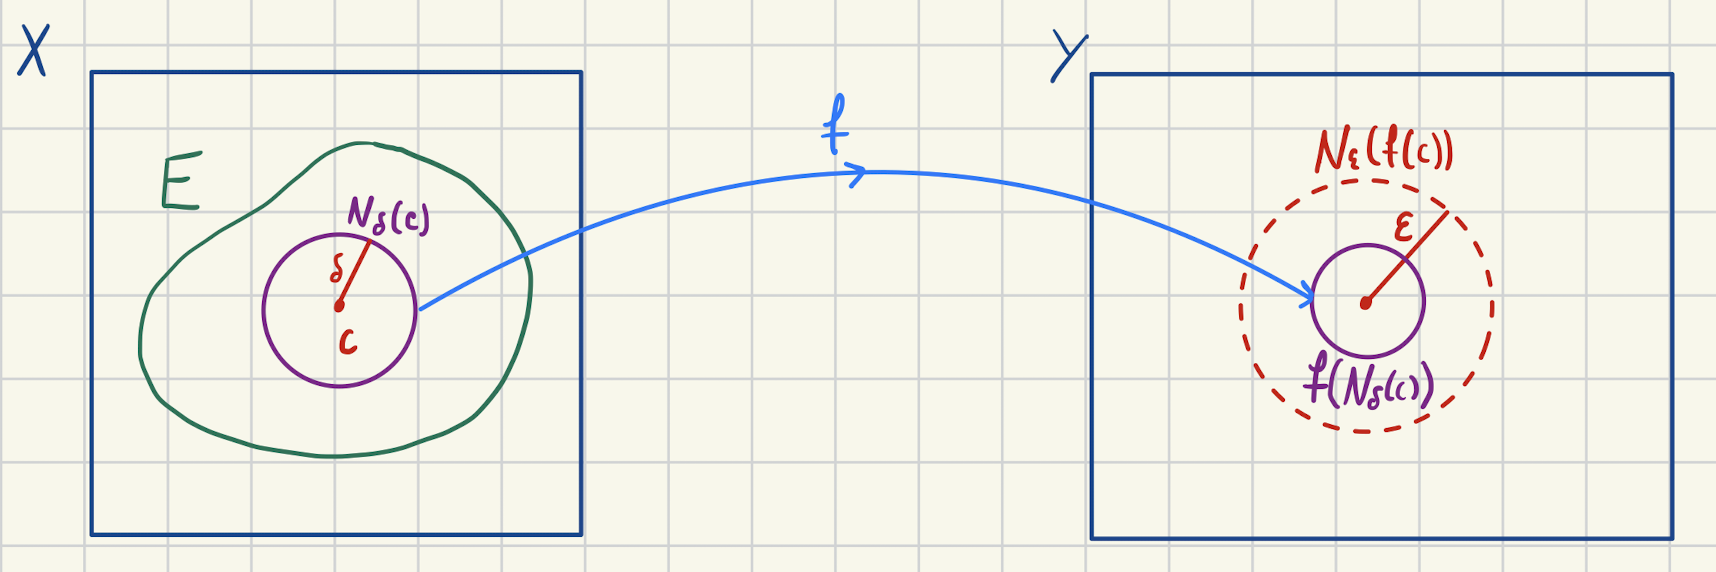
\includegraphics[width=.75\linewidth, center]{/Users/josiahvillarante/GradSchool/Grad-School-Notes/Math230A/Lecture/CH4/images/continuous at c.png}
\end{figure}

\begin{definition}[Continuous Function] \leavevmode \\
    Let $f:E\subseteq X \to Y$. We say $f$ is continuous if it is continuous at every point of $E$.
\end{definition}

\begin{theorem}[Characterization of Continuity via Sequences] \leavevmode \\
    Let $f: E\subseteq X \to Y$. Let $c \in E.$ The following two statements are equivalent:
    \begin{enumerate}[$(i)$]
        \item $f$ is continuous at $c$
        \item For all sequences $(a_n)$ in $E$ satisfying $a_n \to c$ we have $f(a_n) \to f(c)$ 
    \end{enumerate}
\end{theorem}

\begin{proof}
    \begin{description}
        \item[$(i) \implies (ii)$:] \leavevmode \\
        Suppose $f$ is continuous at $c$. Let $(a_n)$ be a sequence in $E$ such that $a_n \to c.$ Our goal is to show that $f(a_n) \to f(c)$, that is, we want to show
        $$\forall \epsilon > 0 ~\exists N \st \forall n > N ~~\overset{\sim}{d}(f(a_n), f(c)) < \epsilon.$$
        Let $\epsilon > 0$ be given. Our goal is to find $N$ such that
        \begin{equation*}
            \text{if $n > N$, then $\overset{\sim}{d}(f(a_n), f(c)) < \epsilon$} \tag{$*$}
        \end{equation*}
        We have
        \begin{enumerate}[$(I)$]
            \item $f$ is continuous at $c \implies \exists \delta > 0 \st \forall x \in \nbhds{\delta}{X}{c}\cap E ~~f(x) \in \nbhds{\epsilon}{Y}{f(c)}$
            \item $a_n \to c \implies \exists \hat{N} \st \forall n > \hat{N} ~~a_n \in \nbhds{\delta}{X}{c}$
        \end{enumerate}
        We claim that we can use $\hat{N}$ as the $N$ that we were looking for. Indeed, if $n > \hat{N}$, then
        \begin{align*}
            (II) \implies
            \begin{rcases*}
                a_n \in \nbhds{\delta}{X}{c} \\
                a_n \in E
            \end{rcases*}
            &\implies a_n \in \nbhds{\delta}{X}{c}\cap E \\
            &\overset{(I)}{\implies} f(a_n) \in \nbhds{\epsilon}{Y}{f(c)}.
        \end{align*}

        \item[$(ii) \implies (i)$:] \leavevmode \\
        Suppose every sequence $(a_n)$ in $E$ such that $a_n \to c$, we have $f(a_n) \to f(c)$. We want to show $f$ is continuous at $c$.
        \begin{info}
            $f$ is continuous at $c \iff \forall \epsilon > 0 ~\exists \delta > 0 \st $ if $x \in \nbhds{\delta}{X}{c}\cap E$ then $f(x) \in \nbhds{\epsilon}{Y}{f(c)}$ \\
            As we discussed last time:
            \begin{enumerate}[$*)$]
                \item if $c \in E \backslash E'$, $f$ is continuous at $c$
                \item if $c \in E'$, then $f$ is continuous at $c \iff \lim \limits_{x \to c}f(x) = f(c)$
            \end{enumerate}
        \end{info}
        We may consider two cases:
        \begin{description}
            \item[Case 1: $c \in E \backslash E'$] ($c$ is an isolated point of $E$) \leavevmode \\
            Any function is continuous at any isolated point of its domain.
            \item[Case 2: $c\in E'$] \leavevmode \\
            It is enough to show that $\lim \limits_{x \to c} f(x) = f(c)$. By the sequential criterion for limits of functions, it is enough to show that
            $$\text{if $(a_n)$ is a sequence in $E \backslash \{c\} \st a_n \to c$, then $f(a_n) \to f(c)$}$$
            But this is a direct consequence of the assumption that
            $$\text{if $(a_n)$ is a sequence in $E \st a_n \to c$, then $f(a_n) \to f(c)$}$$
        \end{description}
    \end{description}
    \qed
\end{proof}

\begin{corollary}[Criterion for Discontinuity]\leavevmode \\
    If you can find one sequence $(a_n)$ in $E$ such that $a_n \to c$, but $f(a_n) \not \to f(c)$, that shows $f$ is not continuous at $c$.
\end{corollary}

\begin{example}
    Prove that the Dirichlet function
    $$f: \R \to \R ~~f(x) = \begin{cases*}
        1 \text{ if } x \in \Q \\
        0 \text{ if } x \not \in \Q
    \end{cases*}$$
    is discontinuous everywhere.
\end{example}

\begin{proof}
    Let $c\in \R$. We will show that $f$ is discontinuous at $c$.
    \begin{description}
        \item[Case 1: $c \in \R \backslash \Q$] ($f(c) = 0$) \leavevmode \\
        Let $(q_n)$ be a sequence of rational numbers such that $q_n \to c.$ Note that
        $$\forall n ~q_n \in \Q \implies \forall n ~f(q_n) = 1 \implies \lim \limits_{n \to \infty}f(q_n) = \lim \limits_{n\to \infty}1 = 1.$$ 
        Therefore,
        $$
        \begin{rcases*}
            q_n \to c \\
            f(q_n) \not \to f(c) = 0
        \end{rcases*} \implies f \text{ is not continuous at $c$}.
        $$
        \item[Case 2: $c \in \Q$] ($f(c) = 1$)\leavevmode \\
        Let $(r_n)$ be a sequence of irrational numbers such that $r_n \to c.$ Note that
        $$\forall n ~r_n \in \R \backslash \Q \implies \forall n ~f(r_n) = 0 \implies \lim \limits_{n\to \infty}f(r_n) = \lim \limits_{n \to \infty}0 = 0.$$
        Therefore,
        $$
        \begin{rcases*}
            r_n \to c \\
            f(r_n) \not \to f(c) = 1
        \end{rcases*} \implies f \text{ is not continuous at $c$}.
        $$
        \qed
    \end{description}
\end{proof}

\begin{example}
    Prove that $f: (\R, d) \to \R$ (where $d$ is the discrete metric) defined by
    $$
    f(x) = \begin{cases*}
        1 &\text{ if $x\in \Q$} \\
        0 &\text{ if $x \not \in \Q$}
    \end{cases*}
    $$
    is continuous everywhere.
\end{example}

\begin{proof}
    Let $c\in \R.$ Our goal is to show that $f$ is coninuous at $c.$ That is, we want to show
    $$\forall \epsilon > 0 ~\exists \delta > 0 \st \text{if $d(x,c) < \delta$, then $|f(x) - f(c)| < \epsilon.$}$$
    Let $\epsilon > 0$ be given. Our goal is to find $\delta > 0$ such that 
    \begin{equation*}
        \text{if $d(x,c) < \delta$, then $|f(x) - f(c)| < \epsilon$}
        \tag{$*$}
    \end{equation*}
    Regardless of the expression of $f$, $(*)$ holds with $\delta = \frac{1}{2}$. Indeed, if $d(x,c) < \frac{1}{2}$, then $d(x,c) = 0,$ so $x=c$ and therefore $|f(x) - f(c)| = 0 < \epsilon,$ as desired. \qed
\end{proof}

\begin{example}
    Let $(X, \|\cdot\|)$ be a normed space. Prove that $\|\cdot\|: X \to \R$ is continuous.
\end{example}

\begin{proof}
    Let $c\in X$. We will prove that $\|\cdot\|$ is continuous at $c.$ That is, we will show
    \begin{equation*}
        \forall \epsilon > 0 ~\exists \delta > 0 \st \text{if $\|x-c\| < \delta$, then $\left|\|x\| - \|c\|\right| < \epsilon$.}
        \tag{$*$}
    \end{equation*}
    It follows immediately from the inequality
    $$\left|\|x\|-\|c\|\right|\leq \|x-c\|$$
    that $(*)$ holds with $\delta = \epsilon.$ \qed
\end{proof}

\begin{corollary}
    If $x_n \to x$ in $X$, then $\|x_n\| \to \|x\|$ in $\R$.
\end{corollary}

\begin{example}
    Let $(X,d)$ be a metric space. Let $p\in X.$ Define $f: X \to \R$ by $f(x) = d(p,x)$. Prove that $f$ is continuous.
\end{example}

\begin{proof}
    Let $c\in X$. our goal is to show that 
    $$\forall \epsilon > 0 ~\exists \delta > 0 \st \text{if $d(x,c) < \delta$, then $|d(p,x) - d(p, c)| < \epsilon.$}$$
    Let $\epsilon > 0$ be given. Our goal is to find $\delta > 0$ such that
    \begin{equation*}
        \text{if $d(x,c) < \delta,$ then $|d(p,x) - d(p,c)| < \epsilon$}
        \tag{$*$}
    \end{equation*}
    It follows immediately from the inequality
    $$|d(p,x) - d(p,c)| \leq d(x,c)$$
    that $(*)$ holds with $\delta = \epsilon.$ \qed
\end{proof}

\begin{example}
    Consider $C[0,1] = \{f:[0,1]\to \R: \text{$f$ is continuous}\}$ equipped with the norm
    $$\|f\|_{\infty} = \max \limits_{0\leq x \leq 1} \left|f(x)\right|.$$
    Prove that $\begin{cases*}
        T: C[0,1] \to \R \\
        T(f) = f(\frac{1}{2})
    \end{cases*}$ is continuous.
\end{example}

\begin{proof}
    Let $g\in C[0,1].$ Our goal is to show that $T$ is continuous at $g$. To this end, it is enough to show that if $g_n \to g$ in $\left(C[0,1], \|\cdot\|_{\infty}\right)$, then $T(g_n) \to T(g)$ in $\R$. We have 
    \begin{align*}
        g_n \to g \text{ in } \left(C[0,1], \| \cdot \|_{\infty}\right)
        &\implies \|g_n - g\|_{\infty} \to 0 \text{ as } n \to \infty \\
        &\implies \max \limits_{0 \leq x \leq 1} \left|g_n(x) - g(x)\right| \to 0 \text{ as } n \to \infty \\
        0 \leq \left|g_n (1/2) - g(1/2)\right| &\leq \max\left|g_n(x) - g(x)\right| \\
        &\implies \left|g_n(1/2) - g(1/2)\right| \to 0 \text{ as } n \to \infty &&\text{(squeeze theorem)} \\
        &\implies g_n(1/2) \to g(1/2) \text{ in } \R \\
        &\implies T(g_n) \to T(g) \text{ in } \R
    \end{align*}
    \qed
\end{proof}

\begin{theorem}[Algebraic Continuity Theorem] \leavevmode \\
    \label{thm4.9}
    Assume $f:E \subseteq (X,d) \to \R$ and $g:E \subseteq (X,d) \to \R$ are continuous at $c\in E$. Then
    \begin{enumerate}[$(i)$]
        \item $kf(x)$ is continuous at $c$ for all $k\in\R$
        \item $f(x) + g(x)$ is continuous at $c$
        \item $f(x)g(x)$ is continuous at $c$
        \item $f(x)/g(x)$ is continuous at $c$ provided $g(c) \not = 0$
    \end{enumerate}
\end{theorem}

\begin{proof} \leavevmode
    These are direct consequences of the algebraic limit theorem for sequences and the characterization of continuity via sequences. For example, let's prove $(iii)$: \\
    By characterization of continuity via sequences, it is enough to show that if $(a_n)$ is a sequence in $E$ such that $a_n \to c$, then $f(a_n)g(a_n) \to f(c)g(c).$ Let $(a_n)$ be such a sequence. We have
    \begin{equation*}
        \begin{rcases*}
            f \text{ is continuous at } c \\
            a_n \to c
        \end{rcases*} \implies f(a_n) \to f(c)
        \tag{$*$}
    \end{equation*}
    \begin{equation*}
        \begin{rcases*}
            g \text{ is continuous at } c \\
            a_n \to c
        \end{rcases*} \implies g(a_n) \to g(c)
        \tag{$**$}
    \end{equation*}
    In what follows from $(*),(**)$, and the algebraic limit theorem for sequences of real numbers that
    $$f(a_n)g(a_n) \to f(c)g(c)$$
    as desired. \qed
\end{proof}

\begin{theorem}[Composition of Continuous Functions is Continuous] \leavevmode \\
    \label{thm4.7}
    Let $(X,d), (Y,\overset{\sim}{d}),$ and $(Z, \overset{\approx}{d})$ be metric spaces. Let $A$ be a nonempty subset of $X$ and $B$ be a nonempty subset of $Y$. Let $f: A \to Y$ and $g: B \to Z$ such that $f(A) \subseteq B.$ Suppose $f$ is continuous at $c \in A$, and $g$ is continuous at $f(c) \in B$. Then $g \circ f: A \to Z$ is continuous at $c \in A$.
\end{theorem}

\begin{proof}
    It is enough to show that if $(a_n)$ is a sequence in $A$ such that $a_n \to c$, then $(g\circ f)(a_n) \to (g \circ f)(c).$ Let $(a_n)$ be such a sequence. We have 
    \begin{align*}
        \begin{rcases*}
            f \text{ is continuous at } c \\
            a_n \to c
        \end{rcases*} &\implies f(a_n) \to f(c) \\
        \begin{rcases*}
            g \text{ is continuous at } f(c) \\
            f(a_n) \to f(c)
        \end{rcases*} &\implies g(f(a_n)) \to g(f(c)).
    \end{align*}
    So, $(g \circ f)(a_n) \to (g \circ f)(c)$ as desired. \qed
\end{proof}

\begin{example}
    If $f: X \to \R$ and $g: X \to \R$ are continuous, then
    $$\text{$\max\{f,g\}$ and $\min\{f,g\}$}$$
    are also continuous.
\end{example}
\begin{align*}
    \max\{a,b\} &= \frac{a+b}{2} + \frac{|a-b|}{2} \\
    \min\{a,b\} &= \frac{a+b}{2} - \frac{|a-b|}{2}
\end{align*}

\begin{example}\leavevmode \\
    \begin{enumerate}[$(1)$]
        \item If $E$ is a metric subspace of $X$, then $$i: E \to X, i(x) = X$$ is continuous.
        \item If $f:X \to Y$ is continuous and $E\subseteq X,$ then $f|_{E}: E \to X$ is continuous.
        \item If $\begin{cases*}
            f: X \to Y \text{ is continuous} \\
            Y \text{ is a metric space}
        \end{cases*}$, then $i \circ f: X \to Z$ is continuous.
    \end{enumerate}
\end{example}